\documentclass[master=mai,masteroption=ecs]{kulemt}
\setup{title={Fixed Size Least Squares Support Vector Machines: A Scala based programming framework for Large Scale Classification},
  author={Mandar Chandorkar},
  promotor={Prof.\,dr.\,ir.\ Bart De Moor \and Prof.\,dr.\,ir.\ Johan A.K Suykens},
  assessor={Ir.\,Kn. Owsmuch\and K. Nowsrest},
  assistant={Oliver Lauwers \and Dr. Raghvendra Mall}}
% The following \setup may be removed entirely if no filing card is wanted
\setup{filingcard,
  translatedtitle=,
  udc=621.3,
  shortabstract={We propose \textit{FS-Scala}, a flexible and modular \textit{Scala} based implementation of the Fixed Size Least Squares Support Vector Machine (FS-LSSVM) for large data sets. The framework consists of a set of modules for (gradient and gradient free) optimization, model representation, kernel functions and evaluation of FS-LSSVM models. A kernel based \textit{Fixed-Size Least Squares Support Vector Machine} (FS-LSSVM) model is implemented in the proposed framework, while heavily leveraging the parallel computing capabilities of \textit{Apache Spark}. Global optimization routines like \emph{Coupled Simulated Annealing} (CSA) and \emph{Grid Search} are implemented and used to tune the hyper-parameters of the FS-LSSVM model. Finally, we carry out experiments on benchmark data sets like \emph{Magic Gamma} and \emph{Adult} and evaluate the performance of various kernel based FS-LSSVM models.}}
% Uncomment the next line for generating the cover page
%\setup{coverpageonly}
% Uncomment the next \setup to generate only the first pages (e.g., if you
% are a Word user.
%\setup{frontpagesonly}

% Choose the main text font (e.g., Latin Modern)
\setup{font=lm}

% If you want to include other LaTeX packages, do it here. 

% Finally the hyperref package is used for pdf files.
% This can be commented out for printed versions.
\usepackage[pdfusetitle,colorlinks,plainpages=false]{hyperref}
\usepackage{blindtext, tikz, csvsimple, adjustbox}
\usepackage{amsmath}
\usepackage{amsfonts}
\usepackage{amssymb}
\interdisplaylinepenalty=2500
\usepackage{tikzscale, adjustbox}

\usepackage[school]{pgf-umlcd}
\usepackage[ruled,vlined,linesnumbered,inoutnumbered]{algorithm2e}
\usepackage{verbatim} 
\usepackage{booktabs} % For \toprule, \midrule and \bottomrule

\usepackage{siunitx} % Formats the units and values
\usepackage{pgfplotstable} % Generates table from .csv
\usepackage{datatool}

\usepackage{textgreek}

\usepackage{times}
%\usepackage{geometry}

\usetikzlibrary{mindmap, backgrounds,positioning,shapes,shadows,arrows}
\sisetup{
  round-mode          = places, % Rounds numbers
  round-precision     = 2, % to 2 places
}

%%%%%%%
% The lipsum package is used to generate random text.
% You never need this in a real master thesis text!
\IfFileExists{lipsum.sty}%
 {\usepackage{lipsum}\setlipsumdefault{11-13}}%
 {\newcommand{\lipsum}[1][11-13]{\par And some text: lipsum ##1.\par}}
%%%%%%%

%\includeonly{chap-n}
\begin{document}

\begin{preface}
  I would like to thank everybody who kept me busy the last year,
  especially my promoter and my assistants. I would also like to thank the
  jury for reading the text. My sincere gratitude also goes to my wife and
  the rest of my family.
\end{preface}

\tableofcontents*

\begin{abstract}
We propose \textit{FS-Scala}, a flexible and modular \textit{Scala} based implementation of the Fixed Size Least Squares Support Vector Machine (FS-LSSVM) for large data sets. The framework consists of a set of modules for (gradient and gradient free) optimization, model representation, kernel functions and evaluation of FS-LSSVM models. A kernel based \textit{Fixed-Size Least Squares Support Vector Machine} (FS-LSSVM) model is implemented in the proposed framework, while heavily leveraging the parallel computing capabilities of \textit{Apache Spark}. Global optimization routines like \emph{Coupled Simulated Annealing} (CSA) and \emph{Grid Search} are implemented and used to tune the hyper-parameters of the FS-LSSVM model. Finally, we carry out experiments on benchmark data sets like \emph{Magic Gamma} and \emph{Adult} and evaluate the performance of various kernel based FS-LSSVM models.
\end{abstract}

% A list of figures and tables is optional
%\listoffigures
%\listoftables
% If you only have a few figures and tables you can use the following instead
\listoffiguresandtables
% The list of symbols is also optional.
% This list must be created manually, e.g., as follows:
\chapter{List of Abbreviations and Symbols}
\section*{Abbreviations}
\begin{flushleft}
  \renewcommand{\arraystretch}{1.1}
  \begin{tabularx}{\textwidth}{@{}p{12mm}X@{}}
    SVM   & Support Vector Machine \\
    FS-LSSVM   & Fixed Size Least Squares Support Vector Machine \\
    CG   & Conjugate Gradient \\
    CSA  & Coupled Simulated Annealing \\
    AFE  & Automatic Feature Extraction \\
    API  & Application Programming Interface \\ 
    KKT  & Karush Kuhn Tucker \\
    RHKS & Reproducing Kernel Hilbert Space\\
    SVC & Support Vector Classification\\
    SVR & Support Vector Regression\\
    SMO & Sequential Minimal Optimization\\
    QP & Quadratic Programming\\
    ROC & Receiver Operating Characteristic\\
    OOP & Object Oriented Programming\\
    FP & Functional Programming\\
    JVM & Java Virtual Machine\\
  \end{tabularx}
\end{flushleft}
\section*{Symbols}
\begin{flushleft}
  \renewcommand{\arraystretch}{1.1}
  \begin{tabularx}{\textwidth}{@{}p{12mm}X@{}}
    42    & ``The Answer to the Ultimate Question of Life, the Universe,
            and Everything'' according to \cite{h2g2} \\
    $c$   & Speed of light \\
    $E$   & Energy \\
    $m$   & Mass \\
    $\pi$ & The number pi \\
  \end{tabularx}
\end{flushleft}

% Now comes the main text
\mainmatter

\chapter{Introduction}
\label{cha:intro}
The $21^{st}$ century stands out in how mankind learned the value of storing and making predictions/decisions from large volumes of data. A significant aspect of large scale data analysis is distributed computation frameworks like \textit{High Performance Computing}, \textit{Message Passing Interface} etc. Recently large scale commodity hardware clusters have replaced the two former frameworks as the most popular model for parallel data analysis. With this crucial change in hardware came a change in computational models as well. It is at this juncture that distributed \textit{Map Reduce} became the de-facto computational philosophy for large scale data analysis and  words such as \textit{Hadoop} \cite{Hadoop:2005}, \cite{chang2008bigtable}, \cite{Borthakur2011} and \textit{Apache Spark} \cite{Zaharia2010}, \cite{Spark:2010} have become synonymous with large scale data analysis and machine learning.

Along with innovation in hardware design and distributed computing models, there came a need for good programming libraries and frameworks to work with various Machine Learning models on large data sets. It was demonstrated in \cite{10.1109/MIS.2009.36} that a gigantic language corpus encapsulates almost all aspects of human language and speech. So far the prevalent `motto' in the Internet industry has been ``large data, simple models". Often, this is misunderstood as the Machine Learning translation of \textit{Occam's Razor}. The bias-variance trade-off \cite{Valentini2004} is a far better mechanism to ensure the model does not become overly complex, and this, rather than restricting the user to simple models, is the real Occam's razor in training a model. 

Therefore, in order to extract maximum value from large scale data, it is important to have the flexibility to train and compare different model families before arriving at the one that fits the requirement of the user. Therefore one must be able to train general nonlinear models and tweak them by changing the various components which they employ to learn (i.e., a model may be linear or kernel based, it can be optimized by various methods like \textit{Stochastic Gradient Descent}, \textit{Conjugate Gradient}, etc.). This is not possible in a rigid, monolithic programming framework. Modularity, extensibility and ease of usage are of paramount importance while designing Machine Learning software for large scale data applications.

Scala \cite{scala-overview-tech-report} a multi-paradigm Java Virtual Machine (JVM) based programming language has gained popularity for its expressiveness and performance. It's power and easy interpolability with Java is has quickly made it the language of choice for production grade Machine Learning software development. The current state of the art in distributed Machine Learning in Scala is the \textit{MLLib} module in \textit{Apache Spark} \cite{Meng}. It has implementations of Linear SVM and Logistic Regression for solving binary classification problems. But a crucial component missing in \textit{MLLib} and all distributed Machine Learning libraries is the ability to learn classification models with nonlinear decision boundaries. FS-Scala aims to solve the problem of scalable non-linear classification models by implementing the \textit{Fixed-Size Least Squares Support Vector Machine} (FS-LSSVM) algorithm \cite{DeBrabanter2010,Suykens2002} with model tuning capabilities.

In recent literature we find sparse reductions to FS-LSSVM methods \cite{Mall2015,Mall2013}. The authors in \cite{Mall2015,Mall2013} explored the sparsity vs error trade-off for FS-LSSVM models. Even though they run experiments on large scale datasets like Forest Cover dataset, the scalability of these methods are restricted to available memory on a single machine. Moreover, they don't exploit the possibility of parallelism available in several components of the FS-LSSVM model. Another work \cite{Mall2014} converts the Big Data into a Big Network and then uses a network based subset selection technique (\textit{Fast and Unique Representative Subset selection} (FURS) \cite{Mall2013FURS}) to obtain a representative subset of the original data. It then builds a FS-LSSVM model using this subset. However, in this thesis we showcase that we can parallelize the subset selection technique which maximizes the \textit{Quadratic R\`enyi Entropy} for Big datasets and use the generated subset as the set of prototype vectors (PV) essential for building the FS-LSSVM model.

%%% Local Variables: 
%%% mode: latex
%%% TeX-master: "thesis"
%%% End: 

\chapter{Least Squares Support Vector Machines}
\label{cha:1}
%%%%%%%%%%%%%%%%%%%%%%%%%%%%%%%%%%%%%%%%%%%
\section{Support Vector Machines} \label{SVM}
 
The classical soft margin Support Vector Machine (SVM) model as proposed by Cortes et. al \cite{Cortes} relies on maximizing the margin between the separating hyper-plane while minimizing the mis-classification error on the input patterns. It is formulated in equation \eqref{eqsvm} below.

\begin{equation}\label{eqsvm}
\begin{aligned}
& \underset{w,b,e}{\text{min}} &
 \mathcal{J}(w,e) = \frac{1}{2}w^{\intercal}w + \gamma\sum\limits_{i=1}^N e_{i} \\
& \text{s.t.} &
y_{i}[ w^{\intercal}\phi(x_{i})+b ] \geq 1 - e_{i},\ i=1,\ldots ,N. \\
& & e_{i} \geq 0,\ i=1,\ldots ,N.
\end{aligned}
\end{equation}

The functions $\phi(x)$ are suitably chosen basis functions, which describe an inner product space called a \textit{Reproducing Kernel Hilbert Space} (RKHS) \cite{N.Aronszjan1950}. The RKHS generated by $\phi(x)$ can be identified by a positive semi-definite Kernel function $K(x, y) = \phi(x)^{T}\phi(y)$, a class of kernel functions popularly known as \textit{Mercer} kernels \cite{Mercer}. Generally the product $\phi(x)^{T}\phi(y)$ is replaced by the Kernel function $K(x, y)$ without explicitly calculating or solving for $\phi(x)$, this is known in SVM literature as the \textit{kernel trick}.

It is well known that solving the optimization problem in equation \eqref{eqsvm} leads to a \textit{sparse} representation of the best separating hyper-plane between the two classes in the data. This can be achieved by introducing Lagrange multipliers and applying the Karush Kuhn Tucker (KKT) conditions yielding a classifier of the form $w = \sum\limits_{k=1}^N \alpha_k y_k \phi(x_{i})$. Most of the multipliers $\alpha_k$ are zero due to the KKT complementary slackness condition, while the non zero multipliers determine the \textit{support vectors}. How ever the classical soft margin SVM formulation also leads to a \textit{Quadratic Programming} (QP) problem in terms of the Lagrange multipliers which often leads to $O(N^3)$ time complexity in the model training.

%%%%%%%%%%%%%%%%%%%%%%%%%%%%%%%%%%%%%%
\section{Least Squares Support Vector Machines}
%%%%%%%%%%%%%%%%%%%%%%%%%%%%%%%%%%%%%%%%%%%
Least Squares Support Vector Machines (LSSVM) proposed by Suykens et.al \cite{Suykens2002, Suykens1999} modify the classical soft margin SVM formulation above by replacing the \textit{hinge} loss function in \eqref{eqsvm} with the \textit{squared error} loss function and the inequality constraints (in terms of the error/slack variables $e_i$) with equality constraints, we obtain the following optimization problem \eqref{eqlssvm}.
\begin{equation}\label{eqlssvm}
\begin{aligned}
& \underset{w,b,e}{\text{min}}
& & \mathcal{J}(w,e) = \frac{1}{2}w^{\intercal}w + \frac{\gamma}{2}\sum\limits_{i=1}^N e_{i}^2 \\
& \text{s.t.}
& & y_{i}[ w^{\intercal}\phi(x_{i})+b ] = 1 - e_{i}, i=1,\ldots ,N.
\end{aligned}
\end{equation}
%%%%%%%%%%%%%%%%%%%%%%%%%%%%%
Introducing the Lagrangian and applying the KKT conditions gives us the solution of the problem in the dual \eqref{eqkkt}.
%%%%%%%%%%%%%%%%%%%%%%%%%%%%%%%%%
\begin{equation}\label{eqkkt}
\left[\begin{array}{c|c}
   0  & y^\intercal   \\ \hline
   y & \Omega + \gamma^{-1} \mathit{I} 
\end{array}\right] 
\left[\begin{array}{c}
   b    \\ \hline
   \alpha  
\end{array}\right] = \left[\begin{array}{c}
   0    \\ \hline
   1_v  
\end{array}\right],
\end{equation}
%%%%%%%%%%%%%%%%%%%%%%%%%%%%%%%%%%%%%%%%%%%%%%%%%%%5
In the above equation, the quantities $\Omega_{kl}$, $\alpha$ and $K(x_k,x_l)$ are given by the following expressions.
\begin{equation*}
\begin{aligned}
& \Omega_{kl} = y_{k}y_{l}K(x_{k}, x_{l}) \\
& \alpha = \left[\alpha_1 ; ... ; \alpha_N \right] \\
& K(x_k,x_l) = \phi(x_k)^\intercal\phi(x_l) \\
\end{aligned}
\end{equation*}

This solution implies a loss of sparsity as compared to the classical SVM since each point becomes a support vector. However, we gain linearity of the solution (i.e. we do not have to solve the \textit{Quadratic Programming} problem as in the classical SVM). This affords us greater freedom in choosing optimization algorithms to solve the formulation in \eqref{eqlssvm}, apart from the standard \textit{Stochastic Gradient Descent} we can also employ algorithms for linear systems such as \textit{Conjugate Gradient}, \textit{Gauss Seidel}, \textit{Jacobi} etc.

%%%%%%%%%%%%%%%%%%%%%%%%%%%%%%%%%%%%%%%%%%%%%%%%%%%%
\section{FS-LSSVM: Tackling Large Scale Problems} \label{sec:fs}
It is observed that solving the problem \eqref{eqkkt} in the dual is not advantageous for large scale analysis as the size of the solution matrix is equal to the size of the original data. In order to make the training of kernel based SVM models for large scale data applications feasible, one must solve the optimization problem in the primal and make approximations to the computation of the kernel matrices. The Fixed-Size LSSVM (FS-LSSVM) as proposed by De Brabanter, Suykens et. al \cite{DeBrabanter2010,Suykens2002} consists of solving the LSSVM problem in the primal as follows. 
%%%%%%%%%%%%%%%%%%%%%%%%%%%%%%

\begin{equation}
\label{eqfs}
\min_{w,b} \ \frac{1}{2}w^{\intercal} w + \frac{\gamma}{2}\sum^{n}_{i=1} \left(y_{i} - w^{\intercal} \hat{\phi}(x_i) - b\right)^{2}.
\end{equation}

The solution to equation \ref{eqfs} is given by:
\begin{align}
\label{eqfssol}
& \left( \begin{matrix}
\hat{w}\\ 
\hat{b}
\end{matrix}\right ) = 
\left ( \hat{\Phi}^{\intercal}_e \hat{\Phi}_e + \frac{\mathit{I}_{m+1}}{\gamma} \right )^{-1} \hat{\Phi}^{\intercal}_e y,
\\ \nonumber \\
\text{where} \hspace{10pt}
& \hat{\Phi}_e = \begin{pmatrix}
\hat{\phi}_{1}(x_1) & \cdots & \hat{\phi}_{m}(x_1) & 1\\ 
\vdots &  \ddots & \vdots & \vdots\\ 
\hat{\phi}_{1}(x_n) & \cdots & \hat{\phi}_{m}(x_n) & 1
\end{pmatrix}. \nonumber
\end{align}

In the above formulation, $\hat{\phi}(x_k)$ is an approximation to the true feature map $\phi(x_k)$ which is related to the kernel $K(x_i, x_j) = \phi(x_i)^{\intercal} \phi(x_j)$ (Mercer's theorem). The approximate feature map $\hat{\phi}(x_k)$ is calculated using the Nystr\"om method as outlined in \cite{DeBrabanter2010, Mall2015, Mall2013}. A low rank approximation to the kernel matrix is constructed by iteratively calculating a subset of the original data which maximizes the \textit{Quadratic R\`enyi Entropy}. This procedure of extracting $\hat{\phi}(x_k)$ from a data set, given a kernel function, is called \textit{Automatic Feature Extraction} (AFE) (see appendix \ref{app:nystrom}).

Kernel based models are sensitive to hyper-parameters. In the case of FS-LSSVM we have to tune the model with respect to $\gamma$ the regularization parameter and the parameters of the kernel chosen. Models are generally compared with their cross-validation performance in which case the objective cost function with respect to the hyper-parameters is in general non-smooth and non-convex. Gradient free methods like Grid Search, Nelder Mead \cite{Nelder1965} and Coupled Simulated Annealing \cite{Xavier-De-Souza2010} are suitable to tackle the problem of model selection for FS-LSSVM based kernel models. Algorithm \ref{lssvmalgo} in appendix \ref{app:n} explains the steps involved in tuning the FS-LSSVM model with the bold part representing our contributions in this thesis, which have been implemented in a \textit{MapReduce} setting.

\chapter{FS-Scala}
\label{cha:2}

\section{Scientific Computing: An Overview}
The term \textit{Scientific Programming} must be interpreted with proper context, as the very first applications of the primitive computational infrastructure developed during the second world war were conducting numerical simulations of various engineering problems of practical significance. It must thus be recognized that only after large scale adoption of computers for business applications became popular, that the term \textit{Scientific Computing} became relevant as a sub-domain of Computer Science.

Nevertheless it is instructive to take a quick glance at the history of programming languages in order to motivate the design philosophy behind \textit{FS-Scala} and the \textit{MapReduce} computational paradigm which has been applied extensively in modern large scale data processing frameworks.

We classify programming languages on two broad issues, for an in-depth treatment of the subject one may refer to some of the canonical texts in the area \cite{Sethi:1989}, \cite{Abelson:1996:SIC:547755}.

\begin{itemize}
\item Translation to Machine level code.
Programs written in any language have to be translated to low level machine readable instructions or codes, this may be achieved in two ways.
\begin{itemize}
\item Compilation: The high level program is "compiled" or translated into low level executable code, this is achieved in various ways on different platforms (i.e. .exe file on Windows based systems, .sh files on *nix systems). Note that this process has to be done once and the executable code can be run many times.

\item Interpretation: Instead of translating the high level code before hand, an interpreter translates all the content of a program into low level instructions every time it is executed.

\end{itemize}

\item Paradigms.

\begin{itemize}
\item Imperative Programming.
Programs consist of instructions which modify a given 'state', which may refer to a memory location or variable.
\item Object Oriented Programming (OOP).
Programs consist of entities called 'objects' which contain data, called 'fields' and subroutines to modify their data.
\item Functional Programming (FP).
Programs consist of expressions which take input and output the results, its worth noting that the input and output data structures are immutable. It is worth noting that in Functional Programming one may pass a function itself as an argument to another function/subroutine, this behavior is colloquially referred to by the phrase "code as data". 
\end{itemize}
\end{itemize}

There are advantages and limitations of each programming language or paradigm, which must be understood before choosing one for a particular application. It is well known that compiled languages have much better performance than interpreted languages, though one must keep in mind that being compiled or interpreted are not inherent characteristics of the languages themselves rather practical implementation details. This advantage that languages like C and Fortran possess is evidenced in the fact that much of the Python scientific programming frameworks use underlying \textit{C} or \textit{Fortran} primitives for fast computation, \textit{scikit-learn} \cite{scikit-learn} being the best example.

So far \textit{Python} and \textit{MATLAB} have been the dominant languages used in computation for engineering and science applications, this is because of their ease of learning with respect to syntax and the ready availability of packages which can be used to extend their capability for specific applications like signal processing (in \textit{MATLAB}) and Natural Language Processing (see \textit{NLTK} \cite{NLTK} ) in \textit{python}.

While \textit{python} and \textit{MATLAB} are convenient for quick prototyping of new algorithms and models, for production machine learning systems their performance makes them unsuitable for those applications. The most common languages used for production systems are \textit{C/C++} and \textit{Java}. 

The Java Virtual Machine (JVM) has become a standard platform for enterprise applications in the past two decades. The \textit{Apache Hadoop} \cite{Hadoop:2005} and \textit{Mahout} \cite{Mahout} big data and machine learning frameworks are written entirely in \textit{Java}. \emph{Apache Mahout} has been applied to large scale problems  \cite{mahoutinaction} of categorization, clustering \cite{mahoutclus} and in recommendation, \cite{mahoutreco1}. 

Apart from \emph{Hadoop} and \emph{Mahout}, other prominent Java machine learning frameworks are \emph{Mallet} \cite{Mallet}, \emph{Deeplearning4j} \cite{dl4j}, \emph{BoofCV} \cite{BoofCV2012}, \emph{MOA} (Massive Online Analysis) \cite{MOA} and \emph{javaML} \cite{javaML} among many others.  As such, the JVM offers a sound platform for future efforts in large scale machine learning. One of the recent developments has been the development of JVM based languages which have embraced the FP paradigm along with the inherent Object Oriented (OO) nature of the \textit{Java} language and the JVM.

\subsection*{Scala, MapReduce and Data Processing}

\textit{Scala} is a hybrid, multi-paradigm language developed at the EPFL, Lausanne in 2004 \cite{scala-overview-tech-report}. It is a JVM based language because all \textit{Scala} code is translated to JVM byte code to be execute like any other Java program. This gives it seamless interpolability with Java and all the programming frameworks written in Java. It is primarily an OOP language which has many functional characteristics like support for \textit{tail recursive} optimization, function composition and immutable data structures. Its is inspired by many prominent FP languages like \textit{Lisp}, \textit{Haskell}, \textit{OCaml} etc.

An important concept or paradigm espoused in many FP languages is \textit{MapReduce}, it can be readily observed that many programs/computations in languages like \textit{Lisp}, \textit{Scala} use \textit{MapReduce} on immutable data structures like lists in order to obtain results. In chapter \ref{cha:3} we delve further into the \textit{MapReduce} paradigm and why it is so central to modern big data architectures. It is instructive to note that in \textit{Scala}, data structures like lists, maps and so on have in built \texttt{map} and \texttt{reduce} functions which enable the programmer to think and code in this paradigm.

It is for these reasons that \textit{Scala} has become crucial to the implementation of modern big data frameworks like \textit{Apache Spark} and the language of choice for us in the implementation of the FS-LSSVM.

\begin{figure}[!ht] 
\begin{adjustbox}{max width=\textwidth}
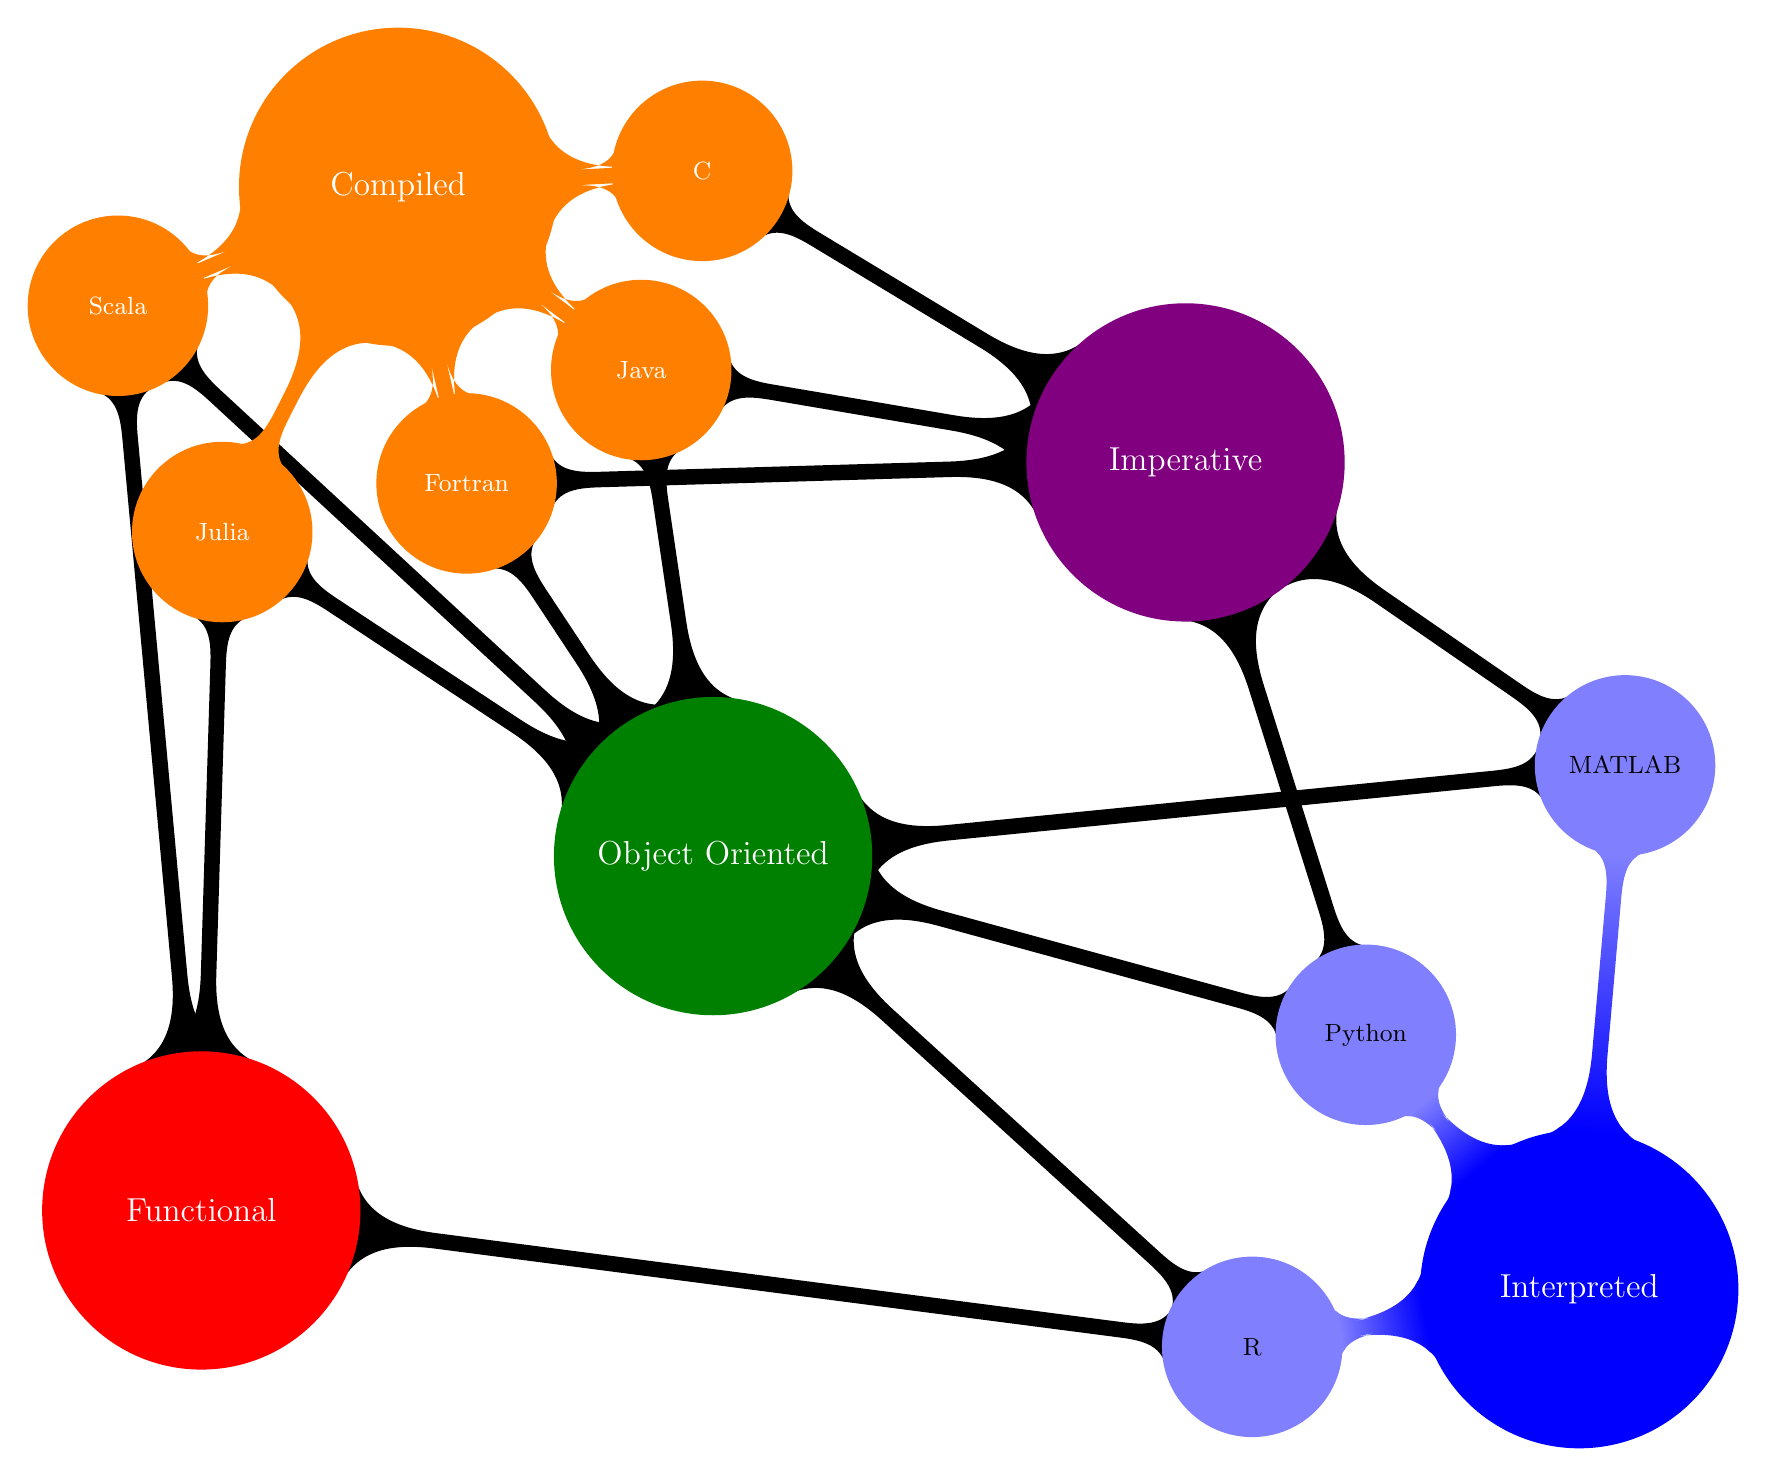
\begin{tikzpicture}[mindmap,
  level 1 concept/.append style={level distance=110,sibling angle=40},
  extra concept/.append style={color=blue!50,text=black}]

  % Applied area: computer science and its subfields

  \begin{scope}[mindmap, concept color=orange, text=white]
    \node [concept] (comp) {Compiled}[clockwise from=3]
        child {node [concept] (c) {C}}
        child {node [concept] (java) {Java}}
        child {node [concept] (fortran) {Fortran}}
        child[level distance=140] {node [concept] (julia) {Julia}}
        child {node [concept] (scala) {Scala}};
  \end{scope}
  
  \begin{scope}[mindmap, concept color=blue]
    \node [concept, text=white] (int) at (15,-14) {Interpreted}
        child [concept color=blue!50, grow=85, level distance=190] 
            {node [concept] (matlab) {MATLAB}}
        child [concept color=blue!50, grow=130, level distance=120] 
            {node [concept] (py) {Python}}
        child [concept color=blue!50, grow=190, level distance=120] 
            {node [concept] (r) {R}};
  \end{scope}

  \begin{scope}[mindmap, concept color=red,text=white]
    \node [concept] (fp) at (-2.5,-13) {Functional};
  \end{scope}

  \begin{scope}[mindmap, concept color=green!50!black,text=white]
    \node [concept] (oop) at (4,-8.5) {Object Oriented};
  \end{scope}

  \begin{scope}[mindmap, concept color=violet, text=white]
    \node [concept] (imp) at (10,-3.5) {Imperative};
  \end{scope}

  \begin{pgfonlayer}{background}
    \path (java) to[circle connection bar] (oop);
    \path (java) to[circle connection bar] (imp);
    \path (scala) to[circle connection bar] (fp);
    \path (scala) to[circle connection bar] (oop);
    \path (c) to[circle connection bar] (imp);
    \path (py) to[circle connection bar] (oop);
    \path (py) to[circle connection bar] (imp);
    \path (r) to[circle connection bar] (fp);
    \path (r) to[circle connection bar] (oop);
    \path (julia) to[circle connection bar] (oop);
    \path (julia) to[circle connection bar] (fp);
    \path (matlab) to[circle connection bar] (oop);
    \path (matlab) to[circle connection bar] (imp);
    \path (fortran) to[circle connection bar] (oop);
    \path (fortran) to[circle connection bar] (imp);
  \end{pgfonlayer}
\end{tikzpicture}
\end{adjustbox}
\caption{Overview of Scientific Computing Languages}
\label{fig:scilang}
\end{figure}

\section{SVM Software: The state of the art}

Since its inception, there have been a number of implementations of the classical soft-margin SVM, one can find a diverse list of software at \cite{SVMSoft}. Notable implementations include \textit{LibSVM} \cite{LibSVM}, \textit{SVM\textsuperscript{Light}} \cite{SVMLight} and \textit{mySVM} \cite{mySVM} among others. With respect to the LSSVM there is an implementation by Suykens et.al \cite{LSSVMLab} called \textit{LSSVMLab} written in \textit{MATLAB}. Below we review salient features of a select subset of SVM software implementations.

\begin{itemize}
\item LibSVM: A C/C++ software package that supports Support Vector Classification (C-SVC and \textnu-SVC),  Regression (\textepsilon-SVR and \textnu-SVR) and Density Estimation. It supports binary as well as multi-class classification. Weighted training for unbalanced data sets, along with support for kernels (precomputed and non precomputed kernel matrices). It also supports Sequential Minimal Optimization (SMO) based training of SVM models. One of the most popular SVM implementations with several language ports and multiple libraries (ex. Scikit Learn \cite{scikit-learn}) which use it as a back-end SVM model builder. 

\item SVM\textsuperscript{Light}: A C based software package that aims to reduce the training times for SVM models using faster optimization algorithms which are achieved by a combination of kernel evaluation caching, heuristics and support vector selection based on \textit{steepest feasible descent}. Recently a new implementation \textit{SVM\textsuperscript{perf}} has also been introduced to further speed up model training compared to \textit{SVM\textsuperscript{light}} for large data sets and to optimize multivariate performance measures like F1 measure, ROC area, etc. For an implementation applicable to structures like trees, one can also use SVM\textsuperscript{struct}. 


\item LSSVMLab: A MATLAB software toolbox to train and test LSSVM models. It has support for kernels as well as Bayesian LSSVM formulations which calculate posterior probability of a model or set of hyper-parameters.

\item Apache Spark SVM: This SVM model implementation exists as a part of the \textit{MLLib} machine learning library in the \textit{Apache Spark} big data and cluster computing platform. It is one of the several linear models that are offered in this libraries. \textit{MLLib} comes bundled with optimization algorithms such as Stochastic Gradient Descent (SGD) \cite{Bottou:2010}  and Limited Memory Broyden-Fletcher-Goldfarb-Shanno (L-BFGS) \cite{Andrew:2007, BFGS}, both methods being iterative require multiple passes through the training data to learn a SVM model instance.

\end{itemize}

\section{FS-Scala: Motivation and Design}
FS-Scala tackles three major issues w.r.t. the implementation of the FS-LSSVM:

\begin{itemize}
\item \textbf{Tuning Kernel Models}:
Since the performance of kernel based models is sensitive with respect to the choice of hyper-parameters, one has to choose a mechanism of model selection or hyper-parameter optimization. In FS-Scala, we implement the Grid Search and Coupled Simulated Annealing global optimization algorithms for model tuning.

\item \textbf{Parallel Computation}\label{mr}:
Big Data analysis requires the distribution of computational work load, \textit{MapReduce} is the dominant paradigm employed for writing distributed data processing programs. In FS-Scala we leverage \textit{MapReduce} to distribute the computation in the pre-processing, training and cross-validation tasks.

\item \textbf{Infrastructure Flexibility}:
The big data landscape has many tools which enable the storage and analysis of large streams of data, they consist of technologies such as, but not limited to \textit{Apache Spark}, \textit{Hadoop}, Graph Databases like \textit{Titan} \cite{Titan:2014}, \textit{OrientDB} \cite{OrientDB:2010}, \textit{Neo4j} \cite{Neo4j:2010}. Creating a powerful framework for model training and evaluation requires the decoupling of storage and processing infrastructure from the actual logic that implements the architecture of learning models.
\end{itemize}

\subsection*{Architecture}
\begin{figure}[!ht] 
\begin{adjustbox}{max width=0.95\textwidth}
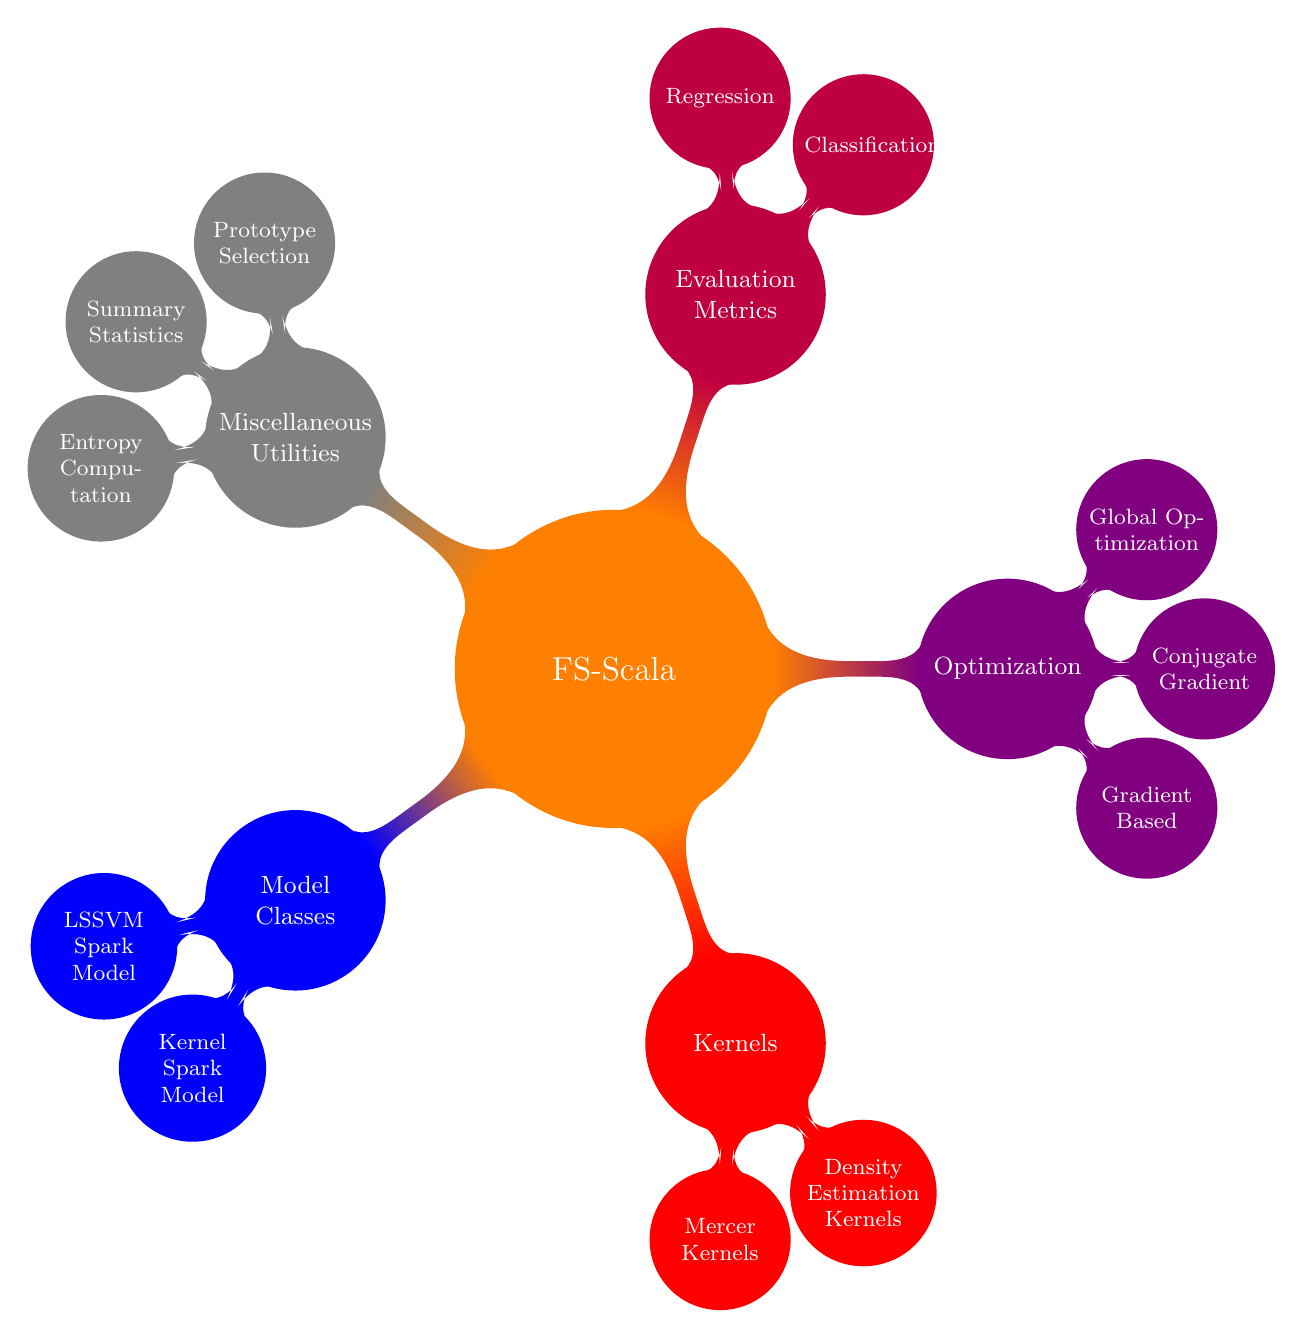
\begin{tikzpicture} [mindmap, grow cyclic, every node/.style=concept, concept color=orange, 
    level 1/.append style={level distance=5cm,sibling angle=72},
    level 2/.append style={level distance=2.5cm,sibling angle=45}, text=white]
\node{FS-Scala}
   child [concept color=blue]{ node {Model Classes}
        child { node {LSSVM Spark Model}}
        child { node {Kernel Spark Model}}
    }
    child [concept color=red]{ node {Kernels}
        child { node {Mercer Kernels}}
        child { node {Density Estimation Kernels}}
    }
    child [concept color=violet]{ node {Optimization}
        child { node {Gradient Based}}
        child { node {Conjugate Gradient}}
        child { node {Global Optimization}}
    }
    child [concept color=purple]{ node {Evaluation Metrics}
        child { node {Classification}}
        child { node {Regression}}
    }
    child [concept color=gray]{ node {Miscellaneous Utilities}
        child { node {Prototype Selection}}
        child { node {Summary Statistics}}
        child { node {Entropy Computation}}
    };

\end{tikzpicture}
\end{adjustbox}
\caption{Schematic structure of FS-Scala}
\label{fig:struct}
\end{figure}

Figure \ref{fig:struct} shows the organization of modules in FS-Scala. It can be decomposed into five principal modules:
\begin{itemize}
\item Model Classes:
This is the core set of classes which form the heart of the library, a number of abstract model categories are defined each with its own set of defined behaviours. 
\item Optimization application programming interface (API):
A module which houses the implementation of common optimization methods (i.e. Gradient and Gradient free). Currently FS-Scala has implementations for Conjugate Gradient, Gradient Descent, Grid Search and Coupled Simulated Annealing \cite{Xavier-De-Souza2010} (CSA). 
\item Kernels:
FS-Scala is equipped with a powerful abstract API for representing kernel functions. The module has two abstract classes to outline the behaviors of kernels used in SVM based applications as well as density estimation. The library comes bundled with an implementation for AFE as well as for common SVM kernels i.e. Linear, Radial Basis Function (RBF), Polynomial, Laplace, Exponential. New kernel functions can be easily added to the library by extending the base classes in this module.
\item Evaluation Metrics:
We have implemented evaluation metrics for Binary Classification and Regression problems. Further more, the implementation of binary classification performance expressed as the area under Receiver Operating Characteristic (ROC), is carried out using \textit{MapReduce} in a \textit{single pass} fashion through the evaluation data points, which can be seen in algorithm \ref{efmr}. Calculating the area under the ROC curve in a \textit{single pass} fashion greatly increases the speed of the eventual FS-LSSVM source code.
\item Miscellaneous Utilities:
This module contains code to carry out auxiliary tasks for model learning and optimization. It contains the implementation of entropy calculation, summary statistics, prototype selection as well as a set of various functions which can be required for implementing new model classes using the library.  

\end{itemize}

\section{Contributions}
\label{contributions}

\subsection{Hyper-parameter tuning}
The modular design approach of FS-Scala provides the user flexibility to apply different tuning algorithms on kernel as well as linear LSSVM models. Kernel based models in FS-Scala all implement the interface \textit{GloballyOptimizable} contained in the optimization module (see Figure \ref{fig:modelUML1} in appendix \ref{app:A}). \textit{GlobalOptimizer} and its subclasses (i.e. \textit{GridSearch} and \textit{CoupledSimulatedAnnealing}) all optimize models which implement the \text{GloballyOptimizable} interface.

\subsection{Speed Improvements}
\begin{itemize}
\item \textbf{Fast Entropy Calculation}:
R\`enyi Entropy based iterative prototype selection is of complexity $O(m^2)$ where $m$ is the number of prototypes to be selected. In FS-Scala after the initial entropy calculation, subsequent computations are only calculated by the entropy difference due to the exchange of one element between the prototype set and rest of the training data. Calculating the entropy differences each iteration is of the order $O(m)$.

\item \textbf{Single Pass Model Training}: 
FS-Scala contains an implementation of CG (algorithm  \ref{cgmr}) which requires only a single pass through the training data to calculate the matrices $A = \left (\hat{\Phi}^{\intercal}_e \hat{\Phi}_e + \frac{\mathit{I}_{m+1}}{\gamma} \right )$ and $c = \hat{\Phi}^{\intercal}_e y$ which are then used to carry out local CG iterations.

\item \textbf{Fast Cross Validation}:
By implementing the fast v-fold cross validation as outlined in \cite{DeBrabanter2010}, FS-Scala eliminates the need to go through the entire training data to calculate the matrices $A_v$ and $c_v$ required for each fold.

\item \textbf{Caching}:
The matrices $A$ and $c$ require a complete pass through the training data to be calculated, but their calculation requires only the original data $(X, Y)$ and the approximate feature map $\hat{\phi}$ which in turn depends on a precomputed kernel matrix with respect to a kernel parameter. By caching the matrices $A$ and $c$ for a particular value of the kernel parameter, FS-Scala can reuse them for multiple values of the regularization parameter $\gamma$. This greatly reduces the total number of passes through the data set the FS-LSSVM algorithm has to carry out, a factor which crucial for tuning of large scale kernel based SVM models.

\end{itemize}

The implementation of the FS-LSSVM in FS-Scala, outlined in algorithm \ref{lssvmalgo}, chapter \ref{cha:1} is as described in in De Brabanter et al. \cite{DeBrabanter2010}.The FS-Scala software is available at \cite{fsscala}.
\chapter{Distributed Computation Support}
\label{cha:3}

\section*{Map Reduce}

As discussed above, we use \textit{MapReduce} wherever possible in order to distribute the workload using \textit{Apache Spark}. Due to the primal formulation of the FS-LSSVM, the size of matrix $A =  \hat{\Phi}^{\intercal}_e \hat{\Phi}_e + \frac{\mathit{I}_{m+1}}{\gamma}$ , in the linear system in \eqref{eqfssol} is $(m+1) \times (m+1)$, where $m$ is the number of prototypes selected to construct the kernel matrix in kernel based FS-LSSVM. Procedure \ref{cgmr} outlines the procedure to estimate the parameters $\hat{w},\ \hat{b}$ of the FS-LSSVM model discussed in section \ref{sec:fs}, using the \textit{Conjugate Gradient} algorithm. 

Using \textit{MapReduce}, we calculate $A = \hat{\Phi}^{\intercal}_e \hat{\Phi}_e + \frac{\mathit{I}_{m+1}}{\gamma}$ and $\hat{\Phi}^{\intercal}_e Y$. We use these results to carry out iterations of the Conjugate Gradient updates until the maximum number of iterations is reached.

\begin{algorithm}[t]\label{fmmr}
    \DontPrintSemicolon
    \KwData{$X = [x^i],\ x^i\ \epsilon \ \mathbf{R}^n$, 
    $\hat{\phi} : \mathbf{R}^n \longrightarrow \mathbf{R}^m$, 
    $Y = [y^i], y^i \epsilon \mathbf{R}$}
    \KwResult{$\left ( \hat{\Phi}^{\intercal}_e \hat{\Phi}_e \right ),\ \hat{\Phi}^{\intercal}_e Y$}
    \Begin{
        $MapFn(x, y)$:\;
        \ \   $M \longleftarrow \hat{\phi}(x) \hat{\phi}(x)^T$\;
        \ \   $v \longleftarrow \hat{\phi}(x) \ y$\;
        $emit(M,v)$\;
    }
    \Begin{
        $RedFn((M, v), (M', v'))$:\;
        $emit(M + M', v + v')$\;
    }
    \Begin{
        $(F, v) \longleftarrow MapReduce(X, MapFn, RedFn)$\;
        
        return $(F, v)$\;
    }
\caption{Calculate feature matrices from data using MapReduce: $FeatureMat$}
\end{algorithm}


\begin{algorithm}[t]\label{cgmr}
    \DontPrintSemicolon
    \KwData{$X = [x^i],\ x^i\ \epsilon \ \mathbf{R}^n$, 
    $\hat{\phi} : \mathbf{R}^n \longrightarrow \mathbf{R}^m$, 
    $Y = [y^i], y^i \epsilon \mathbf{R}$, $\gamma$, $\epsilon$}
    \KwResult{$\left( \begin{matrix}
\hat{w}\\ 
\hat{b}
\end{matrix}\right ) = 
\left ( \hat{\Phi}^{\intercal}_e \hat{\Phi}_e + \frac{\mathit{I}_{m+1}}{\gamma} \right )^{-1} \hat{\Phi}^{\intercal}_e Y$}
    \Begin{
        $(F, v) \longleftarrow FeatureMat(X, Y, \hat{\phi}, \gamma)$ \;
        $A \longleftarrow F + \frac{1}{\gamma} \mathbf{I}_{m \times m}$\;
        \BlankLine
        \nl\While{not $max iterations$ and $\Delta(\hat{w}, \hat{b}) >= \epsilon$}{
            $(\hat{w}_{i+1}, \hat{b}_{i+1}) \longleftarrow CGUpdate(\hat{w}_{i}, \hat{b}_{i}, A, v)$\;
            $\Delta(\hat{w}, \hat{b}) \longleftarrow \left \| \hat{w}_{i+1}  - \hat{w}_{i}\right \|^2 + \left \| \hat{b}_{i+1}  - \hat{b}_{i}\right \|^2$
        }
    }
\caption{Conjugate Gradient: $CG$}
\end{algorithm}


\begin{algorithm}[!htbp]\label{efmr}
    \DontPrintSemicolon
    \KwData{$X_f = [x^i],\ x^i\ \in \ \mathbf{R}^n$, 
    $\hat{\phi} : \mathbf{R}^n \longrightarrow \mathbf{R}^m$, 
    $Y_f = [y^i], y^i \in \mathbf{R}$, $\hat{w}$, $\hat{b}$.}
    \KwResult{score for given fold}
    \Begin{
        $predictLabel(\hat{w}, \hat{b})(x, y)$:\;
        $emit(\hat{w}\cdot x + \hat{b},y)$\;
    }
    \Begin{
        $Vector.fill(length)(IndicatorFn)$:\;
        $vec \longleftarrow (0, ..., 0)_{length} \ map (IndicatorFn)$\;
        $return(vec)$\;
    }
    \Begin{
        $MapScore(score, label)$:\;
        \eIf{label = 1.0}{
            $Pos \longleftarrow Pos + 1$\;
            $tpv \longleftarrow Vector.fill(l)(IndicatorFn(sign(score - thresholds(i)) == 1.0))$\;
            $fpv \longleftarrow Vector.fill(l)(IndicatorFn(false))$\;
        }{
            $Neg \longleftarrow Neg + 1$\;
            $tpv \longleftarrow Vector.fill(l)(IndicatorFn(false))$\;
            $fpv \longleftarrow Vector.fill(l)(IndicatorFn(sign(score - thresholds(i)) == 1.0))$\;
        }
        $emit(tpv,fpv)$\;
    }
    \Begin{
        $RedScore((u, v), (u', v'))$:\;
        $emit(u + u', v + v')$\;
    }
    \Begin{
        $thresholds \longleftarrow List(t_1, t_2, \ldots t_l)$\;
        $Pos \longleftarrow 0$\;
        $Neg \longleftarrow 0$\;
        $scoresLabels \longleftarrow (X_f, Y_f)\ map\ predictLabel(\hat{w}, \hat{b})$\;
        $(tp, fp) \longleftarrow scoresLabels \ map(MapScore) \ reduce(RedScore)$\;
        \BlankLine
        $tp \longleftarrow tp / Pos$
        $fp \longleftarrow fp / Neg$
        $roc \longleftarrow thresholds\ zip(tp\ zip\ fp)$\;
        \BlankLine
        
        return $1 - area(roc)$\;
    }
\caption{Evaluate performance for fold: $evaluateFold$}
\end{algorithm}


\begin{algorithm}\label{cvmr}
    \DontPrintSemicolon
    \KwData{$X = [x^i],\ x^i\ \epsilon \ \mathbf{R}^n$, 
    $\hat{\phi} : \mathbf{R}^n \longrightarrow \mathbf{R}^m$, 
    $Y = [y^i], y^i \epsilon \mathbf{R}$, $\gamma$, folds}
    \KwResult{Cross Validation Performance}
    
    \Begin{
        $(A, v) \longleftarrow FeatureMat(X, Y, \hat{\phi}, \gamma)$ \;
        $score \longleftarrow 0$\;
        \BlankLine
        \nl\For{$i \longleftarrow 1 \ to \ folds $}{
            $(X_i, Y_i) \longleftarrow$ fold i\;
            $(A_i, v_i) \longleftarrow FeatureMat(X_i, Y_i, \hat{\phi}, \gamma)$ \;
            $(\hat{w}, \hat{b}) \longleftarrow CG(A - A_i + \frac{1}{\gamma} \mathbf{I}_{m \times m}, v - v_i)$\;
            $score \longleftarrow score + evaluateFold(\hat{w}, \hat{b}, X_i, Y_i)$\;
        }
        return $score/folds$\;
    }
\caption{Distributed v-Fold Cross-Validation}
\end{algorithm}

% ... and so on until
\npdecimalsign{.}
\nprounddigits{3}
\chapter{Experiments}
\label{cha:n}
The experiments are performed on a 40 core 64GB RAM machine at the Department of Electrical Engineering, KU Leuven. The experiment parameters are summarized in table \ref{table:param}. We use the \textit{Magic Gamma} Telescope, and \textit{Adult} data sets available from the UCI Machine Learning Repository \cite{Lichman:2013}. The performance of various kernel based FS-LSSVM models is carried out for various experimental parameters, each set of experiments is repeated thrice, the mean and standard deviation (in brackets), of the area under ROC curve and the classification accuracy are recorded and presented in tables \ref{table1} and \ref{table2}.

\begin{itemize}
\item Magic Gamma: The data is generated by the registration of high speed gamma particles measured by a ground based atmospheric Cherenkov gamma telescope. Each entry consists of 10 numerical attributes and a binary class attribute. 
\item Adult: This is based on a a census study carried out in 1994, the data consists of 6 numerical attributes and 8 categorical attributes. The target attribute is binary class value, which indicates if the given individual has an annual income more than $50 000$\$.
\item Forest Cover Type: This consists of cartographic data collected by the US Forest Service (USFS) on $30 \times 30$ metre cells which have can have seven different forest cover types. For the purposes of the experiments below, a binary classification problem is constructed which consists of recognizing cover type class two from the other cover types. 
\end{itemize}

\begin{table*}[!htbp]
\caption{Experiment Parameters}
\label{table:param}
\centering
\adjustbox{max width=\textwidth}{
\begin{tabular}{ |c|c| }
\hline
Name & Meaning \\
\hline
Kernel & The type of kernel used i.e. RBF, Polynomial, etc \\ 
Prototypes & Size of prototype set \\ 
Global Opt. & Hyper-parameter optimization algorithm i.e. gs: Grid Search, csa: Coupled Simulated Annealing \\
Grid Size & Number of points (per hyper-parameter) in the grid  \\
Grid Resolution & Distance between two adjacent points on each axis of the grid \\
Accuracy & Classification accuracy on test set. \\
F1 score & avg. F1 score \\
ROC area & avg. area under the ROC curve \\
\hline
\end{tabular}
}
\end{table*}

%\begin{table}[!t]
%% increase table row spacing, adjust to taste
%\renewcommand{\arraystretch}{1.3}
% if using array.sty, it might be a good idea to tweak the value of
% \extrarowheight as needed to properly center the text within the cells
%\caption{An Example of a Table}
%\label{table_example}
%\centering
%% Some packages, such as MDW tools, offer better commands for making tables
%% than the plain LaTeX2e tabular which is used here.
%\begin{tabular}{|c||c|}
%\hline
%One & Two\\
%\hline
%Three & Four\\
%\hline
%\end{tabular}
%\end{table}



The performance of binary FS-LSSVM classifiers on the \textit{MAGIC Gamma} Telescope Data Set obtained from the UCI Machine Learning Repository, are summarized in Table \ref{table1}. FS-LSSVM models trained with polynomial kernels give better classification performance than the RBF and Linear counterparts, on the \textit{MAGIC Gamma} data.

\DTLloaddb{magicgamma}{resultsMagicGammaProc.csv}
\begin{table*}[!htbp]
\sisetup{round-mode=places}
\caption{Magic Gamma Test Results}
\begin{center}
\adjustbox{max width=\textwidth}{
\begin{tabular}{|l|l|l|l|l|l|l|l|l|}\label{table1}
\bfseries Kernel & \bfseries Prototypes & \bfseries Global Optimization & \bfseries Grid Size & 
\bfseries Grid Resolution & \bfseries Accuracy & \bfseries F1 score & \bfseries ROC area & \bfseries Execution Time%
\DTLforeach{magicgamma}{\kernel=kernel,\prototypes=prototypes,
\globaloptimization=globaloptimization,\gridsize=gridsize,
\gridresolution=gridresolution,\acc=accuracy,\stdA=stdA,\maxF=maxF1score,
\stdF=stdF,\areaunderROC=areaunderROC,\stdR=stdR,\time=time,\stdT=stdT}%
{%
  \\\kernel & \prototypes & \globaloptimization & \gridsize & \gridresolution & 
  $\acc(\stdA)$ & $\maxF(\stdF)$ & $\areaunderROC(\stdR)$ & $\time(\stdT)$
}%
\end{tabular}
}
\end{center}
\end{table*}

The performance of binary FS-LSSVM classifiers on the \textit{Adult} Data Set, are summarized in Table \ref{table2}. FS-LSSVM models trained with exponential kernels give better classification performance than the RBF and Linear counterparts, on the \textit{Adult} data. For both the data sets one sees a pattern emerging that tuning kernel models with CSA gives better results than naive \textit{Grid Search} based hyper-parameter optimization.

\DTLloaddb{adultres}{adultres.csv}
\begin{table*}[!htbp]
\caption{Adult Data Set Test Results}
\begin{center}
\adjustbox{max width=\textwidth}{
\begin{tabular}{|l|l|l|l|l|l|l|l|l|}\label{table2}
\bfseries Kernel & \bfseries Prototypes & \bfseries Global Optimization & \bfseries Grid Size & 
\bfseries Grid Resolution & \bfseries Accuracy & \bfseries F1 score & \bfseries ROC area & \bfseries Execution Time%
\DTLforeach{adultres}{\kernel=kernel,\prototypes=prototypes,
\globaloptimization=globaloptimization,\gridsize=gridsize,
\gridresolution=gridresolution,\acc=accuracy,\stdA=stdA,\maxF=maxF1score,
\stdF=stdF,\areaunderROC=areaunderROC,\stdR=stdR,\time=time,\stdT=stdT}%
{%
  \\\kernel & \prototypes & \globaloptimization & \gridsize & \gridresolution & 
  $\acc(\stdA)$ & $\maxF(\stdF)$ & $\areaunderROC(\stdR)$ & $\time(\stdT)$
}%
\end{tabular}
}
\end{center}
\end{table*}

\DTLloaddb{forestcoverproc}{forestcoverproc.csv}
\begin{table*}[!htbp]
\caption{Forest Cover Type Data Set Test Results}
\begin{center}
\adjustbox{max width=\textwidth}{
\begin{tabular}{|l|l|l|l|l|l|l|l|l|}\label{table3}
\bfseries Kernel & \bfseries Prototypes & \bfseries Global Optimization & \bfseries Grid Size & 
\bfseries Grid Resolution & \bfseries Accuracy & \bfseries F1 score & \bfseries ROC area & \bfseries Execution Time%
\DTLforeach{forestcoverproc}{\kernel=kernel,\prototypes=prototypes,
\globaloptimization=globaloptimization,\gridsize=gridsize,
\gridresolution=gridresolution,\acc=accuracy,\stdA=stdA,\maxF=maxF1score,
\stdF=stdF,\areaunderROC=areaunderROC,\stdR=stdR,\time=time,\stdT=stdT}%
{%
  \\\kernel & \prototypes & \globaloptimization & \gridsize & \gridresolution & 
  $\acc(\stdA)$ & $\maxF(\stdF)$ & $\areaunderROC(\stdR)$ & $\time(\stdT)$
}%
\end{tabular}
}
\end{center}
\end{table*}

%%% Local Variables: 
%%% mode: latex
%%% TeX-master: "thesis"
%%% End: 

\chapter{Conclusion}
\label{cha:conclusion}
In this thesis \textit{FS-Scala}, a Scala-based implementation for training and tuning kernel based FS-LSSVM models. As a use case, the kernel based FS-LSSVM model is tested on benchmark data sets. We observed that our implementation enables scalable training, tuning and evaluation of models learning from Big Data, while still providing flexibility to tweak various underlying data processing infrastructure.



%%% Local Variables: 
%%% mode: latex
%%% TeX-master: "thesis"
%%% End: 


% If you have appendices:
\appendixpage*          % if wanted
\appendix
\chapter{FS-Scala Class Hierarchies}
\label{app:A}
Figures \ref{fig:modelUML} and \ref{fig:modelUML1} depict the class hierarchy structures of the core and optimization modules respectively, we can discuss their role in depth.

\section{Core Components}
The core module consists of a set of classes which all originate from a base abstraction called \textit{Model}. It also has classes \textit{ParameterizedLearner} and \textit{LinearModel} representing the core behaviors of parameter based Machine Learning models which form a large chunk of current learning techniques. By using generic typing inherent in the Scala language, one is able to separate the logic of a model from the details of the underlying data infrastructure. This is particularly relevant due to the explosion of data processing frameworks and systems like graph databases, Apache Spark, key value stores, column oriented databases, etc.

\subsection*{Kernel Functions and Kernel Based Models}
The kernel module contains implementations of SVM kernels and AFE. The class \textit{KernelizedModel} defines kernel based linear models which use the \textit{GlobalOptimizer} class to tune values of hyper-parameters. The actual implementation of the \textit{Automatic Feature Extraction} is abstracted out in the parent classes, thereby reducing the effort of writing new SVM kernels to merely expressing their evaluation functions.


\begin{figure}[!ht]
\begin{adjustbox}{max width=0.85\textwidth}
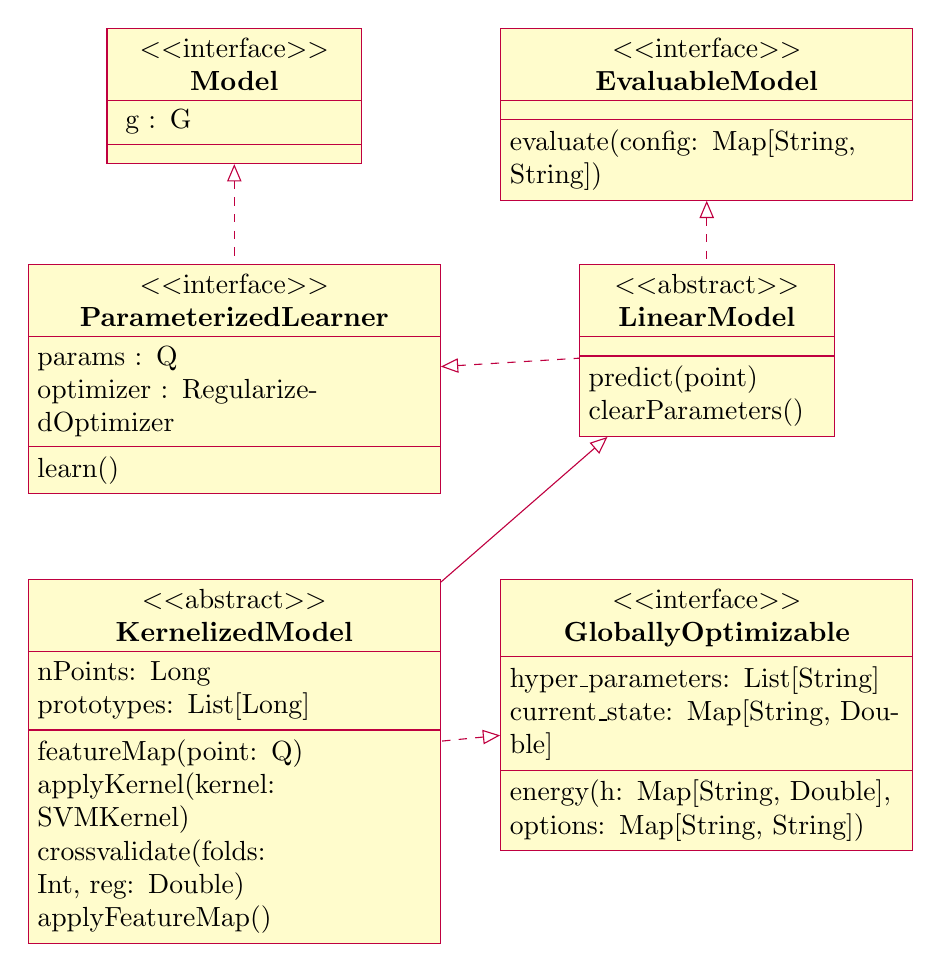
\begin{tikzpicture}
    \begin{interface}[text width =3 cm]{Model}{0 ,0}
        \attribute { g : G }
    \end{interface}
    
    \begin{interface}[]{ParameterizedLearner}{ 0 , -3}
        \implement{Model}
        \attribute{params : Q}
        \attribute{optimizer : RegularizedOptimizer}
        \operation{learn() }
    \end{interface}
    
    \begin{interface}[]{EvaluableModel}{ 6 , 0}
        \operation{evaluate(config: Map[String, String]) }
    \end{interface}
    
    \begin{abstractclass}[text width =3 cm]{LinearModel}{6 , -3}
        \implement{ParameterizedLearner}
        \implement{EvaluableModel}
        \operation{predict(point) }
        \operation{clearParameters() }
    \end{abstractclass}
    
    \begin{interface}[]{GloballyOptimizable}{ 6 , -7}
        \attribute{hyper\_parameters: List[String]}
        \attribute{current\_state: Map[String, Double]}
        \operation{energy(h: Map[String, Double], options: Map[String, String]) }
    \end{interface}
    
    \begin{abstractclass}[]{KernelizedModel}{0 , -7}
        \inherit{LinearModel}
        \implement{GloballyOptimizable}
        \attribute{nPoints: Long}
        \attribute{prototypes: List[Long]}
        \operation{featureMap(point: Q)}
        \operation{applyKernel(kernel: SVMKernel) }
        \operation{crossvalidate(folds: Int, reg: Double)}
        \operation{applyFeatureMap()}
    \end{abstractclass}
    
\end{tikzpicture}
\end{adjustbox}
\caption{Class Hierarchy of Core Models API}
\label{fig:modelUML}
\end{figure}

\section{Optimization Methods}
Parametric models in FS-Scala have an embedded optimization object which is inherits from the \textit{Optimizer} interface. Implementations of Conjugate Gradient and Gradient Descent are provided in the optimization module. New optimization algorithms can be added by inheriting from the top level \textit{Optimizer} interface or the \textit{RegularizedOptimizer} abstract class in case one is working with parametric models which involve regularization. Another important component of the optimization module is the \textit{GlobalOptimizer} interface which acts as a skeleton for implementing gradient free global optimization algorithms.

\begin{figure}[!ht]
\begin{adjustbox}{max width=0.85\textwidth}
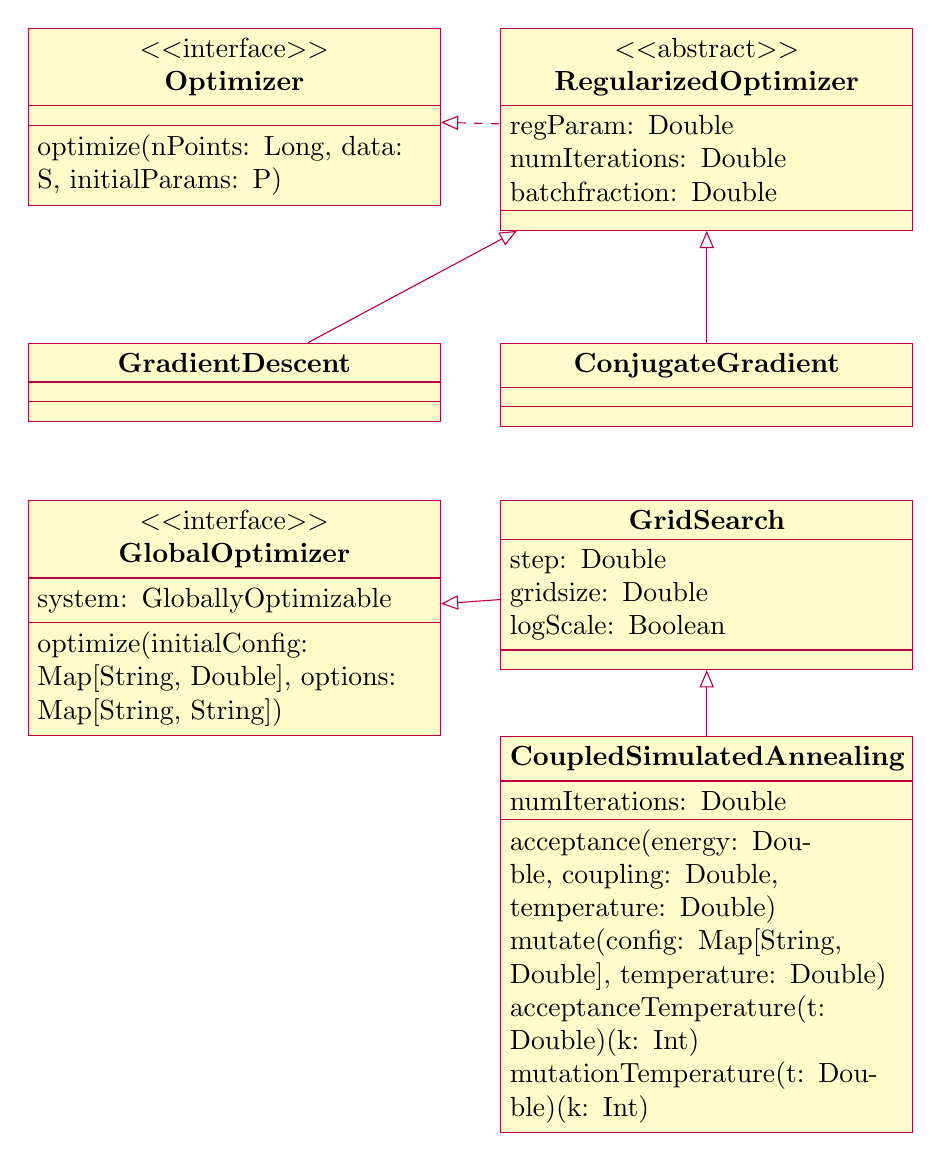
\begin{tikzpicture}
    \begin{interface}[]{Optimizer}{0 ,0}
        \operation{optimize(nPoints: Long, data: S, initialParams: P)}
    \end{interface}
    
    \begin{abstractclass}[]{RegularizedOptimizer}{6 , 0}
        \implement{Optimizer}
        \attribute{regParam: Double}
        \attribute{numIterations: Double}
        \attribute{batchfraction: Double}
    \end{abstractclass}
    
    \begin{class}[]{GradientDescent}{ 0 , -4}
        \inherit{RegularizedOptimizer}
    \end{class}
    
    \begin{class}[]{ConjugateGradient}{6 , -4}
        \inherit{RegularizedOptimizer}
    \end{class}
    
    \begin{interface}[]{GlobalOptimizer}{ 0 , -6}
        \attribute{system: GloballyOptimizable}
        \operation{optimize(initialConfig: Map[String, Double], options: Map[String, String])}
    \end{interface}
    
    \begin{class}[]{GridSearch}{6 , -6}
        \inherit{GlobalOptimizer}
        \attribute{step: Double}
        \attribute{gridsize: Double}
        \attribute{logScale: Boolean}
    \end{class}
    
    \begin{class}[]{CoupledSimulatedAnnealing}{6 , -9}
        \inherit{GridSearch}
        \attribute{numIterations: Double}
        \operation{acceptance(energy: Double, coupling: Double, temperature: Double)}
        \operation{mutate(config: Map[String, Double], temperature: Double)}
        \operation{acceptanceTemperature(t: Double)(k: Int)}
        \operation{mutationTemperature(t: Double)(k: Int)}
    \end{class}
    
    
    
\end{tikzpicture}
\end{adjustbox}
\caption{Class Hierarchy of Optimization API}
\label{fig:modelUML1}
\end{figure}


%%% Local Variables: 
%%% mode: latex
%%% TeX-master: "thesis"
%%% End: 

% ... and so on until
\backmatter
% The bibliography comes after the appendices.
% You can replace the standard "abbrv" bibliography style by another one.
\bibliographystyle{abbrv}
\bibliography{references}

\end{document}

%%% Local Variables: 
%%% mode: latex
%%% TeX-master: t
%%% End: 
